\chapter{Metode Penelitian}

\section{Desain Penelitian}

\vspace{-.5cm}
\begin{figure}[h!]
  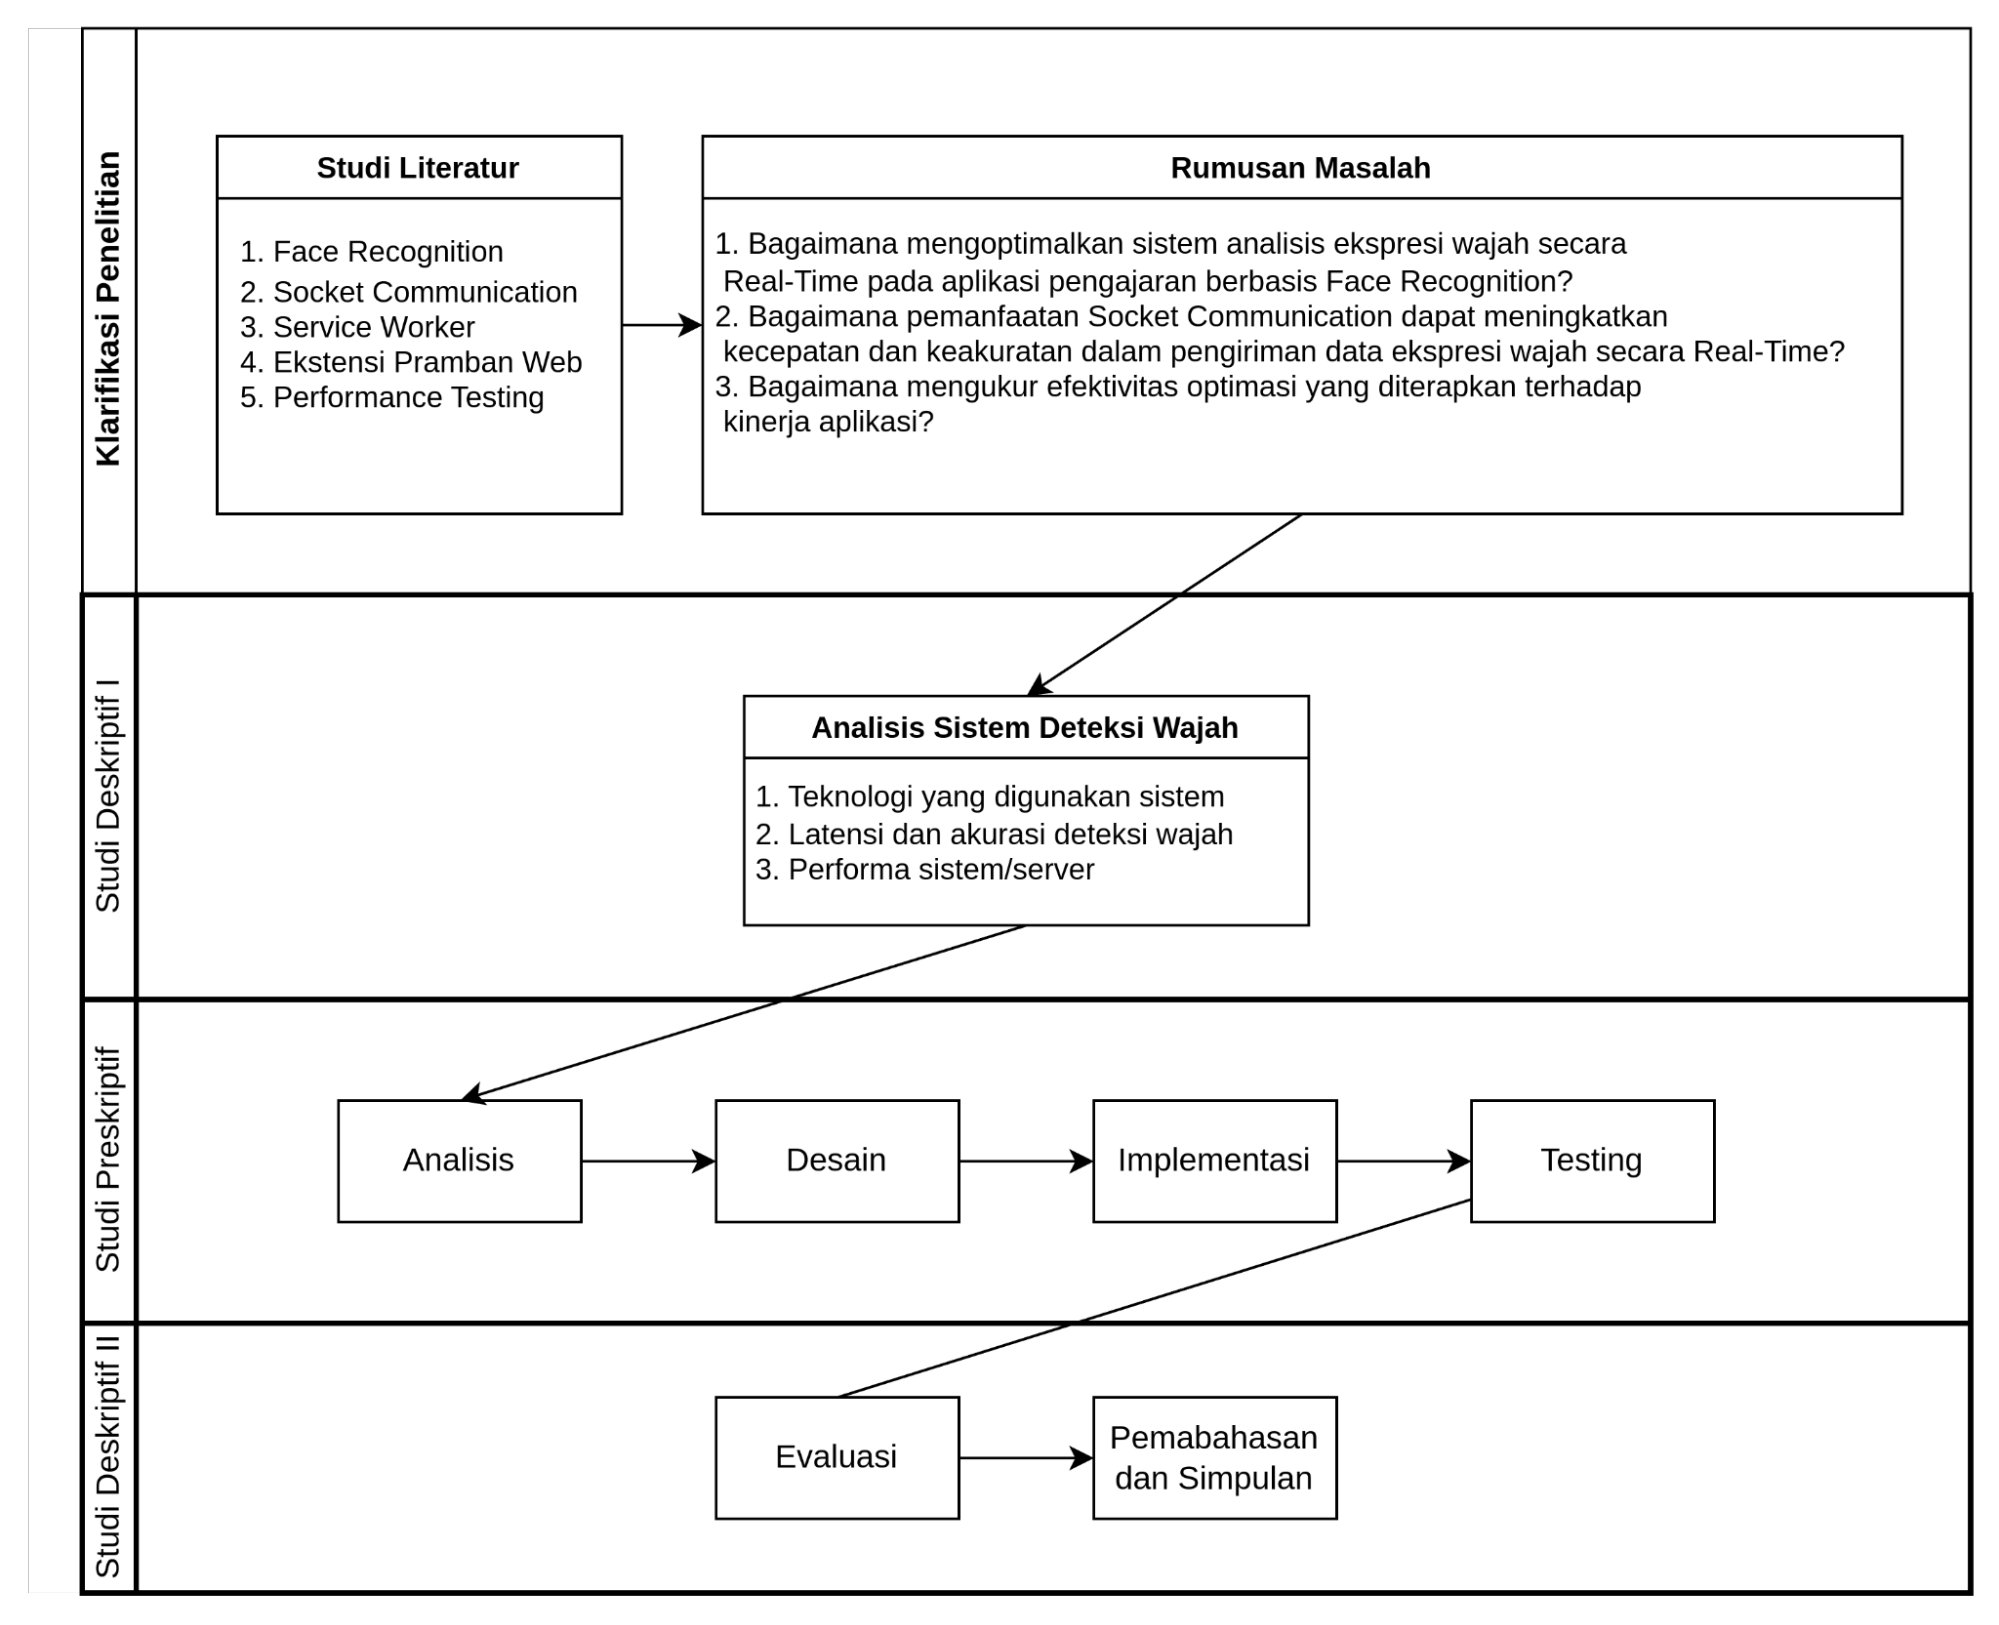
\includegraphics[
    width=14.5cm,
    height=13.5cm,
  ]{images/drm.png}
  \caption{Design Research Methodology (DRM)}
\end{figure}

Penelitian ini menggunakan pendekatan Design Research Methodology (DRM) untuk mengembangkan solusi teknis secara sistematis.
Tujuan utamanya adalah merancang, mengimplementasikan, dan mengevaluasi arsitektur sistem untuk aplikasi EMODU di Google Cloud Platform (GCP).
Melalui DRM, penelitian berfokus pada perancangan arsitektur yang memenuhi tiga pilar utama: ketersediaan tinggi (\textit{high availability}), skalabilitas otomatis (\textit{scalability}), dan penerapan tanpa henti (\textit{zero-downtime deployment}).

\subsection{Klarifikasi Penelitian}
Tahap ini berfokus pada identifikasi masalah dan penentuan ruang lingkup penelitian.
Masalah utama yang diidentifikasi adalah bagaimana membangun infrastruktur yang andal dan efisien untuk aplikasi EMODU, yang berpotensi mengalami pertumbuhan pengguna dan beban kerja yang fluktuatif.
Ruang lingkup penelitian dibatasi pada perancangan dan implementasi arsitektur di Google Cloud Platform (GCP).
Kajian pustaka akan difokuskan pada konsep-konsep kunci seperti arsitektur \textit{high availability}, mekanisme \textit{scalability} pada GCP (misalnya, Managed Instance Groups), strategi \textit{zero-downtime deployment} (seperti Blue-Green atau Rolling Updates), dan praktik terbaik DevOps untuk CI/CD.

\subsection{Studi Deskriptif I}
Pada tahap ini, dilakukan analisis terhadap arsitektur awal atau baseline dari aplikasi EMODU.
Tujuannya adalah untuk memahami komponen-komponen sistem yang ada (backend NestJS, CMS Next.js, komunikasi socket) dan mengidentifikasi potensi kelemahan infrastruktur.
Analisis ini mencakup identifikasi titik tunggal kegagalan (\textit{single points of failure}), potensi masalah skalabilitas, dan proses deployment yang masih manual.
Hasil dari studi ini akan menjadi dasar untuk perancangan arsitektur yang lebih tangguh dan otomatis.

\subsection{Studi Preskriptif}
Pada tahap ini, dirancang sebuah arsitektur infrastruktur solusi di Google Cloud Platform (GCP) untuk mengatasi masalah yang telah diidentifikasi.
Desain arsitektur akan merinci penggunaan layanan-layanan GCP yang spesifik, seperti Google Compute Engine dengan Managed Instance Groups untuk \textit{scaling}, Cloud Load Balancing untuk distribusi lalu lintas dan \textit{high availability}, serta Cloud Build atau GitHub Actions untuk membangun pipeline CI/CD yang mendukung \textit{zero-downtime deployment}.
Arsitektur ini dirancang secara eksplisit untuk memastikan sistem dapat pulih dari kegagalan, beradaptasi dengan beban pengguna, dan dapat diperbarui tanpa mengganggu layanan.

\subsection{Studi Deskriptif II}
Pada tahap ini, arsitektur yang telah dirancang akan diimplementasikan dan dievaluasi kinerjanya.
Aplikasi EMODU akan di-deploy pada infrastruktur GCP yang baru, kemudian serangkaian pengujian akan dilakukan untuk memvalidasi pencapaian tujuan penelitian.
Evaluasi akan mencakup:
\begin{itemize}
    \item \textbf{Pengujian High Availability:} Melakukan simulasi kegagalan (contoh: menghentikan salah satu instance server) dan mengukur waktu pemulihan sistem secara otomatis.
    \item \textbf{Pengujian scalability:} Menggunakan alat \textit{load testing} seperti JMeter untuk memberikan beban lalu lintas yang tinggi dan memverifikasi bahwa sistem secara otomatis menambah atau mengurangi jumlah instance sesuai dengan beban.
    \item \textbf{Pengujian Zero-Downtime Deployment:} Menjalankan pipeline deployment untuk versi baru aplikasi dan memverifikasi bahwa tidak ada gangguan layanan atau kegagalan permintaan selama proses pembaruan.
\end{itemize}
Hasil dari evaluasi ini akan menunjukkan efektivitas dari arsitektur yang diimplementasikan.

\section{Populasi dan Sampel}
Fokus penelitian ini adalah pada sistem teknis, bukan pada pengguna manusia.
Dengan demikian, \textbf{populasi} dalam penelitian ini adalah keseluruhan kemungkinan konfigurasi arsitektur infrastruktur untuk aplikasi berskala seperti EMODU.
\textbf{Sampel} yang diambil adalah arsitektur spesifik yang dirancang dan diimplementasikan pada Google Cloud Platform dalam penelitian ini.
Objek yang diuji bukanlah partisipan manusia, melainkan kinerja dari komponen-komponen infrastruktur itu sendiri ketika diberikan beban kerja yang disimulasikan.

\section{Alat dan Bahan Penelitian}
\subsection{Alat Penelitian}
Spesifikasi komputer yang digunakan untuk pengembangan dan pengelolaan adalah sebagai berikut:
\begin{itemize}
  \item CPU AMD Ryzen 5 PRO 5650U
  \item RAM 14.94 GB
  \item SSD 256 GB
\end{itemize}

\hspace{-32pt} Perangkat lunak yang akan digunakan dalam penelitian ini meliputi:
\begin{itemize}
  \item Fedora Workstation 41
  \item Node.js, NestJS, ReactJS (untuk aplikasi EMODU)
  \item Docker (untuk kontainerisasi aplikasi)
  \item Google Cloud SDK (gcloud CLI)
  \item Postman (untuk pengujian API)
  \item JMeter (untuk \textit{load testing})
  \item Playwright (untuk pengujian \textit{end-to-end})
  \item Grafana \& Google Cloud Monitoring (untuk observabilitas dan visualisasi metrik)
  \item GitHub Actions (untuk pipeline CI/CD)
  \item Zotero, LaTex, Visual Studio Code
\end{itemize}

\hspace{-32pt} Infrastruktur \textit{cloud} yang digunakan dalam penelitian ini adalah \textbf{Google Cloud Platform (GCP)}. Layanan utama yang akan digunakan meliputi:
\begin{itemize}
  \item \textbf{Google Compute Engine (GCE):} Sebagai penyedia mesin virtual untuk menjalankan aplikasi.
  \item \textbf{Managed Instance Groups (MIGs):} Untuk mengelola grup instance dan menerapkan \textit{scaling}.
  \item \textbf{Cloud Load Balancing:} Untuk mendistribusikan lalu lintas dan menyediakan satu titik akses yang \textit{highly available}.
  \item \textbf{Cloud Build:} Sebagai platform CI/CD untuk otomatisasi build, test, dan deploy.
  \item \textbf{Artifact Registry:} Untuk menyimpan dan mengelola artefak build seperti image Docker.
\end{itemize}

\subsection{Bahan Penelitian}
Bahan penelitian yang digunakan meliputi sumber-sumber literatur teknis, yaitu: artikel jurnal ilmiah, dokumentasi resmi dari Google Cloud Platform, buku, dan panduan praktik terbaik (\textit{best practices}) yang berkaitan dengan arsitektur \textit{high availability}, \textit{scalability}, dan \textit{zero-downtime deployment}.
Selain itu, data utama yang menjadi bahan penelitian adalah data kuantitatif berupa metrik kinerja sistem (misalnya, waktu respons, tingkat kesalahan, utilisasi CPU, jumlah instance) yang dikumpulkan dari hasil pengujian beban dan pemantauan sistem.

\section{Instrumen Penelitian}
Instrumen yang digunakan dalam penelitian ini adalah alat untuk membangun, mengukur, dan mengevaluasi arsitektur sistem.
Instrumen utama adalah \textbf{arsitektur infrastruktur itu sendiri} yang diimplementasikan di GCP.
Untuk mengukur kinerja arsitektur tersebut, digunakan instrumen-instrumen berikut:
\begin{itemize}
    \item \textbf{JMeter dan Playwright:} Digunakan sebagai instrumen \textit{load testing} untuk menghasilkan beban pengguna sintetis dan mengukur metrik kinerja seperti \textit{throughput} dan latensi.
    \item \textbf{Google Cloud Monitoring dan Grafana:} Digunakan sebagai instrumen observabilitas untuk mengumpulkan, memantau, dan memvisualisasikan data metrik dari infrastruktur secara \textit{real-time}, seperti utilisasi CPU, jumlah instance, dan status \textit{health check}.
    \item \textbf{Pipeline CI/CD (GitHub Actions/Cloud Build):} Digunakan sebagai instrumen untuk menguji dan memvalidasi proses \textit{zero-downtime deployment}.
    \item \textbf{Skrip Otomatisasi:} Skrip yang dibuat untuk mensimulasikan kegagalan (fault injection), misalnya mematikan instance secara acak, untuk menguji mekanisme \textit{high availability} dan \textit{-failover}.
\end{itemize}
Kombinasi instrumen ini memungkinkan pengumpulan data yang objektif untuk mengevaluasi keberhasilan implementasi arsitektur.

\section{Analisis Data}
Analisis data dalam penelitian ini bersifat kuantitatif dan berfokus pada metrik kinerja infrastruktur yang telah dikumpulkan.
Data akan dianalisis untuk mengevaluasi setiap tujuan utama penelitian:
\begin{itemize}
    \item \textbf{Analisis Scalability:} Menganalisis grafik korelasi antara peningkatan beban (jumlah pengguna virtual) dengan metrik seperti waktu respons dan jumlah instance server yang aktif. Keberhasilan dinilai dari kemampuan sistem menjaga waktu respons tetap stabil dengan menyesuaikan jumlah instance secara otomatis.
    \item \textbf{Analisis High Availability:} Menganalisis log dan data monitoring untuk mengukur waktu yang dibutuhkan sistem untuk pulih setelah simulasi kegagalan. Keberhasilan diukur dari kecepatan pemulihan dan minimnya tingkat kesalahan selama proses \textit{failover}.
    \item \textbf{Analisis Zero-Downtime Deployment:} Menganalisis metrik ketersediaan (availability) dan tingkat kesalahan (error rate) selama proses deployment. Keberhasilan dinilai jika metrik menunjukkan 100\% ketersediaan dan 0\% kesalahan selama pembaruan berlangsung.
\end{itemize}
Hasil analisis ini akan menjadi dasar untuk menarik kesimpulan mengenai efektivitas arsitektur yang diusulkan dalam mencapai \textit{high availability}, \textit{scalability}, dan \textit{zero-downtime deployment}.
